\documentclass[conference]{IEEEtran}
\IEEEoverridecommandlockouts
\usepackage{cite}
\usepackage{amsmath,amssymb,amsfonts}
\usepackage{algorithm}
\usepackage{algpseudocode}
\usepackage{graphicx}
\usepackage{booktabs}
\usepackage{multirow}
\usepackage{xcolor}
\usepackage{url}
\graphicspath{{../docs/figures/}}

\begin{document}

\title{SHADE: Knapsack-Dual Admission and Eviction for CDN Edge Caches, with a Frozen-Method Evaluation on Real Traces}

\author{
\IEEEauthorblockN{Member 1, Member 2, Member 3, Member 4}
\IEEEauthorblockA{\textit{Course: Design and Analysis of Algorithms}\\
\textit{Department, Institution}\\
City, Country}
}

\maketitle

\begin{abstract}
A CDN edge server must decide which objects to keep and which newly requested objects are worth storing at all.
Offline, this is a knapsack problem over \emph{reuse intervals}: covering an interval earns one hit and costs
\emph{size}$\times$\emph{gap} units of cache space-time. Its fractional relaxation is solved by the greedy rule and,
by LP duality, the optimum is a threshold on hit density set by a single shadow price. We present SHADE
(Shadow-price Admission and hit-Density Eviction), an online policy that estimates reuse-time distributions for all
recently seen objects (with Kaplan--Meier censoring, exponential forgetting and empirical-Bayes shrinkage), ranks
objects by an optimal-stopping hit-density index, and admits a new object only if it wins a knapsack exchange test
against the objects it would displace. We evaluate SHADE in simulation on three public Wikimedia CDN traces (90M
requests in total) against eight policies we reimplemented, with the method frozen on a separate development slice
before any held-out run. SHADE has the lowest object miss ratio in 12 of 15 held-out settings, with 6--8\% fewer
misses than the strongest baseline (GDSF) at small and medium cache sizes on the two media traces. It is clearly
worse than GDSF at the largest cache size (by 18--24\%). Its byte-objective variant gains only 0.3--1.9\% over
S3-FIFO. All results come from a single simulation run per setting, from one operator's traffic, without learned
baselines. We also describe the knapsack solver library from an earlier version of the project, and a negative result:
an exact per-epoch knapsack planner that won on synthetic traffic did not carry over to real traffic.
\end{abstract}

\begin{IEEEkeywords}
caching, content delivery networks, knapsack problem, LP duality, online algorithms, admission control
\end{IEEEkeywords}

%=====================================================================
\section{Introduction}
An edge cache of capacity $C$ bytes sees a stream of requests for objects whose sizes span several orders of
magnitude. On each miss it fetches the object from the origin and must decide whether to store it
(\emph{admission}) and, if space is needed, what to remove (\emph{eviction}). In our traces 53--68\% of objects
are requested exactly once, so storing every miss wastes space on objects that will never be hit; CDNs use rules such as cache-on-second-hit for this reason \cite{akamai}.

This work started as a course project in Design and Analysis of Algorithms. The first version (v1) treated caching
as a 0/1 knapsack solved exactly every epoch over forecast popularity, and built a library of knapsack solvers for
it. That planner beat all baselines on synthetic workloads, but it did not carry over to real traffic
(Section~\ref{sec:v1}). The second version keeps the knapsack view but applies it to reuse intervals, following
Berger et al.~\cite{pfoo}, and turns the resulting threshold structure into an online policy.

\textbf{Contributions.} (1) SHADE, an online policy that uses one learned density for both eviction and admission,
learned from all recently requested objects rather than only cached ones. (2) An evaluation protocol in which the
method is frozen on a development slice before any held-out run, with eight reimplemented baselines, an offline
upper bound, and ablations. (3) A library of nine knapsack solvers and a multiple-choice knapsack, with measured
complexity, as the algorithmic foundation. (4) An explicit account of where the method loses and of the threats to
validity.

We do \emph{not} claim a theoretical guarantee (such as a competitive ratio) for SHADE, and we have not done an
exhaustive literature search on its novelty.

%=====================================================================
\section{Background and Related Work}
\textbf{Classic policies.} LRU and FIFO ignore size and frequency. LRU is $k$-competitive for uniform sizes
\cite{sleator}. Belady's rule \cite{belady} is optimal offline for uniform sizes but not for variable sizes, where
offline optimal caching is NP-hard \cite{pfoo}.
\textbf{Size-aware and frequency-aware policies.} GDSF \cite{gdsf} ranks by frequency$\times$cost/size with an
aging term. AdaptSize \cite{adaptsize} admits objects with probability $e^{-\text{size}/c}$ and tunes $c$ with a
Markov model. LHD \cite{lhd} ranks by hit density, estimated from objects in the cache. W-TinyLFU \cite{tinylfu}
admits by a frequency sketch. S3-FIFO \cite{s3fifo} and SIEVE \cite{sieve} are recent simple FIFO-based policies.
\textbf{Learned policies.} LRB \cite{lrb} approximates relaxed Belady with gradient-boosted trees. We do not compare
against learned policies.
\textbf{Bounds.} Berger et al.~\cite{pfoo} formulate caching as a min-cost flow and give the PFOO-L bound, a
fractional knapsack over reuse intervals. Our derivation in Section~\ref{sec:formulation} restates it.

%=====================================================================
\section{Problem Formulation}\label{sec:formulation}
Let the trace be requests $r_1,\dots,r_N$ for objects with sizes $s_x$. For each request $i$ with next request to
the same object at $\mathrm{next}(i)$, define a reuse interval of length $D_i=\mathrm{next}(i)-i$ (logical time,
counted in requests). Keeping the object across the interval yields one hit and uses $s_x D_i$ of space-time.
The cache offers $C N$ space-time in total. Selecting intervals to maximise hits is
\begin{equation}
\max \sum_i y_i \quad \text{s.t.} \quad \sum_i s_{x(i)} D_i\, y_i \le C N,\; y_i\in\{0,1\}.
\label{eq:kp}
\end{equation}
This drops the per-instant constraint that occupancy never exceeds $C$, so it is a relaxation of caching.
Relaxing $y_i\in[0,1]$ gives a fractional knapsack, solved exactly by sorting intervals by density
$1/(s_x D_i)$ and filling greedily. This is the PFOO-L bound \cite{pfoo}; we use it as a lower bound on any
policy's miss ratio.

\textbf{Threshold structure.} Let $\lambda$ be the dual variable of the space-time constraint. By complementary
slackness, the optimum covers interval $i$ iff $1/(s_x D_i) > \lambda$ (one break item may be fractional). The
offline optimum is therefore a threshold on hits per byte per unit time. SHADE tries to approximate this rule
online, where $D_i$ is unknown.

%=====================================================================
\section{SHADE}
\subsection{Learning reuse-time distributions}
SHADE records, for every object requested in the last $2^{23}$ requests (cached or not), its request count $k$ and
the gap $g$ between its last two requests. These define a class $c=(\mathrm{bucket}(k),\lfloor\log_2 g\rfloor)$,
208 classes in total. When an object is requested again, its reuse age is added to a histogram for the class it
had at its previous request. Three statistical corrections are applied:
\begin{itemize}
\item \emph{Censoring.} Objects still waiting for a reuse are counted as censored at their current age, and the
hazard $h_c(a)$ is estimated Kaplan--Meier style as reuses at age $a$ divided by objects at risk at age $a$.
Counting only completed reuses would bias estimates toward short reuse times.
\item \emph{Forgetting.} Statistics decay with a half-life of $2^{22}$ requests. Every interval is weighted by its
start time, so decay does not bias long intervals.
\item \emph{Shrinkage.} Sparse (class, age) cells are shrunk toward the parent class (same count bucket) and then the
global hazard, with 8 pseudo-observations per level.
\end{itemize}
Because these statistics include uncached objects, SHADE can value an object \emph{before} admitting it. LHD, which
learns only from cached objects, cannot.

\subsection{Optimal-stopping index}
Let $S_c(a)$ be the survival function (probability of no reuse by age $a$) for class $c$. Holding an object of
age $a$ for up to $\tau$ more steps gives expected hits $(S_c(a)-S_c(\tau))/S_c(a)$ at expected holding time
$\sum_{t=a}^{\tau-1}S_c(t)/S_c(a)$. SHADE uses the best ratio over all horizons:
\begin{equation}
I(c,a)=\max_{\tau>a}\frac{S_c(a)-S_c(\tau)}{\sum_{t=a}^{\tau-1}S_c(t)},\qquad
\mathrm{rank}(x)=\frac{I(c_x,a_x)}{s_x}.
\end{equation}
This is the online counterpart of the density $1/(s_x D)$. With a decreasing hazard it reduces to the hazard
itself. Taking the maximum over $\tau$ avoids a fixed-horizon parameter and values reuse distributions with a later
second peak, which we observed in the Wikipedia data near $2^{17}$--$2^{21}$ requests (plausibly daily cycles; we did
not verify the cause). The table $I(c,a)$ is refitted every $2^{18}$ requests in
$O(|\mathcal{C}|\cdot A^2)$ time for $A$ age buckets (about 2M operations).

\subsection{Eviction and admission}
Algorithm~\ref{alg:shade} summarises the request path. Eviction samples 32 cached objects, merges them with a pool
of 32 low-ranked candidates kept from earlier evictions, and evicts the lowest rank. Admission applies the exchange
argument from the greedy knapsack proof: a new object replaces its victims only if its rank exceeds every victim's
rank by a margin $m$. We use $m=2$, the method's only tuned constant, chosen on the development slice. The margin is
needed because a new object's index is an estimate at age $0$.

\begin{algorithm}[t]
\caption{SHADE request handling}\label{alg:shade}
\begin{algorithmic}[1]
\Procedure{Request}{$x$}
  \State update count, gap, class and reuse histograms for $x$
  \If{$x$ is cached} \State \Return HIT \EndIf
  \If{free space $\ge s_x$} \State insert $x$; \Return MISS \EndIf
  \State $V\gets\emptyset$
  \While{free space $+\sum_{v\in V}s_v < s_x$}
     \State $v\gets$ lowest-rank object in (32 samples $\cup$ pool)
     \State $V\gets V\cup\{v\}$
  \EndWhile
  \If{$\mathrm{rank}(x)\ge m\cdot\max_{v\in V}\mathrm{rank}(v)$}
     \State evict all $v\in V$; insert $x$
  \EndIf \Comment{otherwise serve $x$ without storing it}
  \State \Return MISS
\EndProcedure
\end{algorithmic}
\end{algorithm}

\subsection{Cost}
Per request: $O(1)$ bookkeeping plus ranking 32--64 candidates on eviction (table lookups). Memory: about 12 bytes
per object seen in the window plus 8 bytes per request in the window ($2^{23}$ requests $\approx$ 64\,MB). This is
more metadata than LRU or S3-FIFO; bounding it with a ghost table was not evaluated. Simulation speed was
0.3--2\,$\mu$s per request.

\subsection{What is borrowed}
The knapsack view and threshold structure come from PFOO \cite{pfoo}; hit density as a rank and sampled eviction
from LHD \cite{lhd}; the eviction pool from Redis; the estimators are standard statistics. The parts we believe are
new are the combination of (i) one density used for both eviction and admission through the exchange test,
(ii) policy-independent, censoring-corrected statistics over all recent objects, and (iii) the optimal-stopping
index. The ablation (Section~\ref{sec:ablation}) shows that (i), as a separate test, contributes little.

%=====================================================================
\section{Knapsack Solver Library (v1)}\label{sec:solvers}
The v1 planner solved a 0/1 knapsack (item = object, weight = size, value = forecast benefit) every epoch. We
implemented the solvers in Table~\ref{tab:solvers} (Hirschberg-style space reduction \cite{hirschberg}, the Martello--Toth bound \cite{mt}, an Ibarra--Kim style FPTAS \cite{ibarra}) in C++17 and tested every exact solver against brute force on
600 random instances.

\begin{table}[t]
\centering
\caption{Implemented knapsack solvers (v1)}\label{tab:solvers}
\begin{tabular}{@{}lll@{}}
\toprule
Algorithm & Time & Space \\
\midrule
2-D DP & $\Theta(nC)$ & $\Theta(nC)$ \\
Rolling DP + bit table & $\Theta(nC)$ & $\Theta(C)$ words + $nC$ bits \\
Hirschberg-style D\&C DP & $\Theta(nC)$ & $\Theta(n+C)$ \\
Branch \& bound (MT bound) & $O(2^n)$ worst & $O(n)$ \\
Meet-in-the-middle & $O(n2^{n/2})$ & $O(2^{n/2})$ \\
FPTAS ($\ge(1-\varepsilon)$OPT) & $O(n^2/\varepsilon)$ & $O(n^2/\varepsilon)$ bits \\
Greedy / modified greedy & $O(n\log n)$ & $O(n)$ \\
Multiple-choice KP DP & $O(C\sum_g|g|)$ & $O(C+GC)$ \\
\bottomrule
\end{tabular}
\end{table}

Measured results: at $n=8000$, $C=8192$ the 2-D table needs 512\,MB, the rolling DP 8\,MB and the Hirschberg-style DP
159\,KB, with the same $\Theta(nC)$ time growth. Fitted log-log slopes of time versus $n$ were 0.7--1.2 for the DPs and
2.09 for the FPTAS. On strongly correlated instances branch and bound reached its $5\cdot10^7$-node cap at $n=200$,
while the DP took 15\,ms. Meet-in-the-middle solved $n=40$ at $C\approx10^{10}$ in 563\,ms. The FPTAS's observed error
($\le$0.09\% for $\varepsilon\le0.1$) was far below its guarantee. The recursive branch and bound overflowed the
stack on real-trace instances; we replaced it with an iterative version. These are benchmarks of our implementations
on our machine, not comparisons with optimised solvers.

%=====================================================================
\section{Experimental Methodology}
\textbf{Traces.} Three public traces (Table~\ref{tab:traces}): the Wikipedia 2018 trace from the LRB paper
\cite{lrb}, and day~1 of the Wikimedia 2019 upload (media) and text (HTML) traces.
\begin{table}[t]
\centering
\caption{Traces. ``Once'' = share of objects requested once.}\label{tab:traces}
\begin{tabular}{@{}lrrrr@{}}
\toprule
Trace & Requests & Objects & Footprint & Once \\
\midrule
W18 dev (req.\ 0--10M) & 10.0M & 2.0M & 191\,GB & 62\% \\
W18 test (req.\ 10--50M) & 40.0M & 4.5M & 503\,GB & 55\% \\
W19 upload, day 1 & 40.0M & 6.9M & 610\,GB & 53\% \\
W19 text, day 1 & 10.2M & 3.7M & 89\,GB & 68\% \\
\bottomrule
\end{tabular}
\end{table}

\textbf{Protocol.} All design choices and the margin $m=2$ were decided on the W18 development slice. The SHADE code
was committed before the held-out runs, and the policy source files are unchanged between that commit and the
results commit. We note that this commit order is the only evidence: the protocol was not externally
pre-registered, and the same authors ran both phases on the same day.
The W18 test slice is from the same trace as the development slice (the following 40M requests), so it is less
independent than the two 2019 traces.

\textbf{Baselines.} LRU, FIFO, SIEVE \cite{sieve}, S3-FIFO \cite{s3fifo}, GDSF \cite{gdsf}, W-TinyLFU \cite{tinylfu},
AdaptSize \cite{adaptsize}, and LHD \cite{lhd}, all in the same simulator. LHD is ported from the authors'
MIT-licensed code; the others are our reimplementations with default parameters from their papers. We did not
validate them against the original implementations' outputs, so a weaker-than-published baseline is possible. One
sign of this: AdaptSize's miss ratio is almost flat between 0.1\% and 0.3\% cache on the development slice.

\textbf{References.} The PFOO-L bound (a true lower bound on miss ratio) and Belady-Size, an offline heuristic with
future knowledge (not optimal for variable sizes).

\textbf{Metrics and setup.} Object and byte miss ratio over the whole trace, cold start included. Cache sizes are
0.1\%, 0.3\%, 1\%, 3\% and 10\% of each trace's footprint. Time is logical (request count), as in \cite{lhd,pfoo}.
\textbf{Each setting was run once with seed 42.} SHADE and LHD use random sampling, so run-to-run variance exists,
but we did not measure it and report no confidence intervals.

\textbf{Correctness checks.} 460 automated checks pass, including: no policy exceeds capacity, no policy hits on a
first request, and no policy (offline references included) beats the PFOO-L bound.

%=====================================================================
\section{Results}
\subsection{Object miss ratio}
Fig.~\ref{fig:miss} and Table~\ref{tab:main} compare SHADE with the best baseline at each setting.

\begin{figure*}[t]
\centering
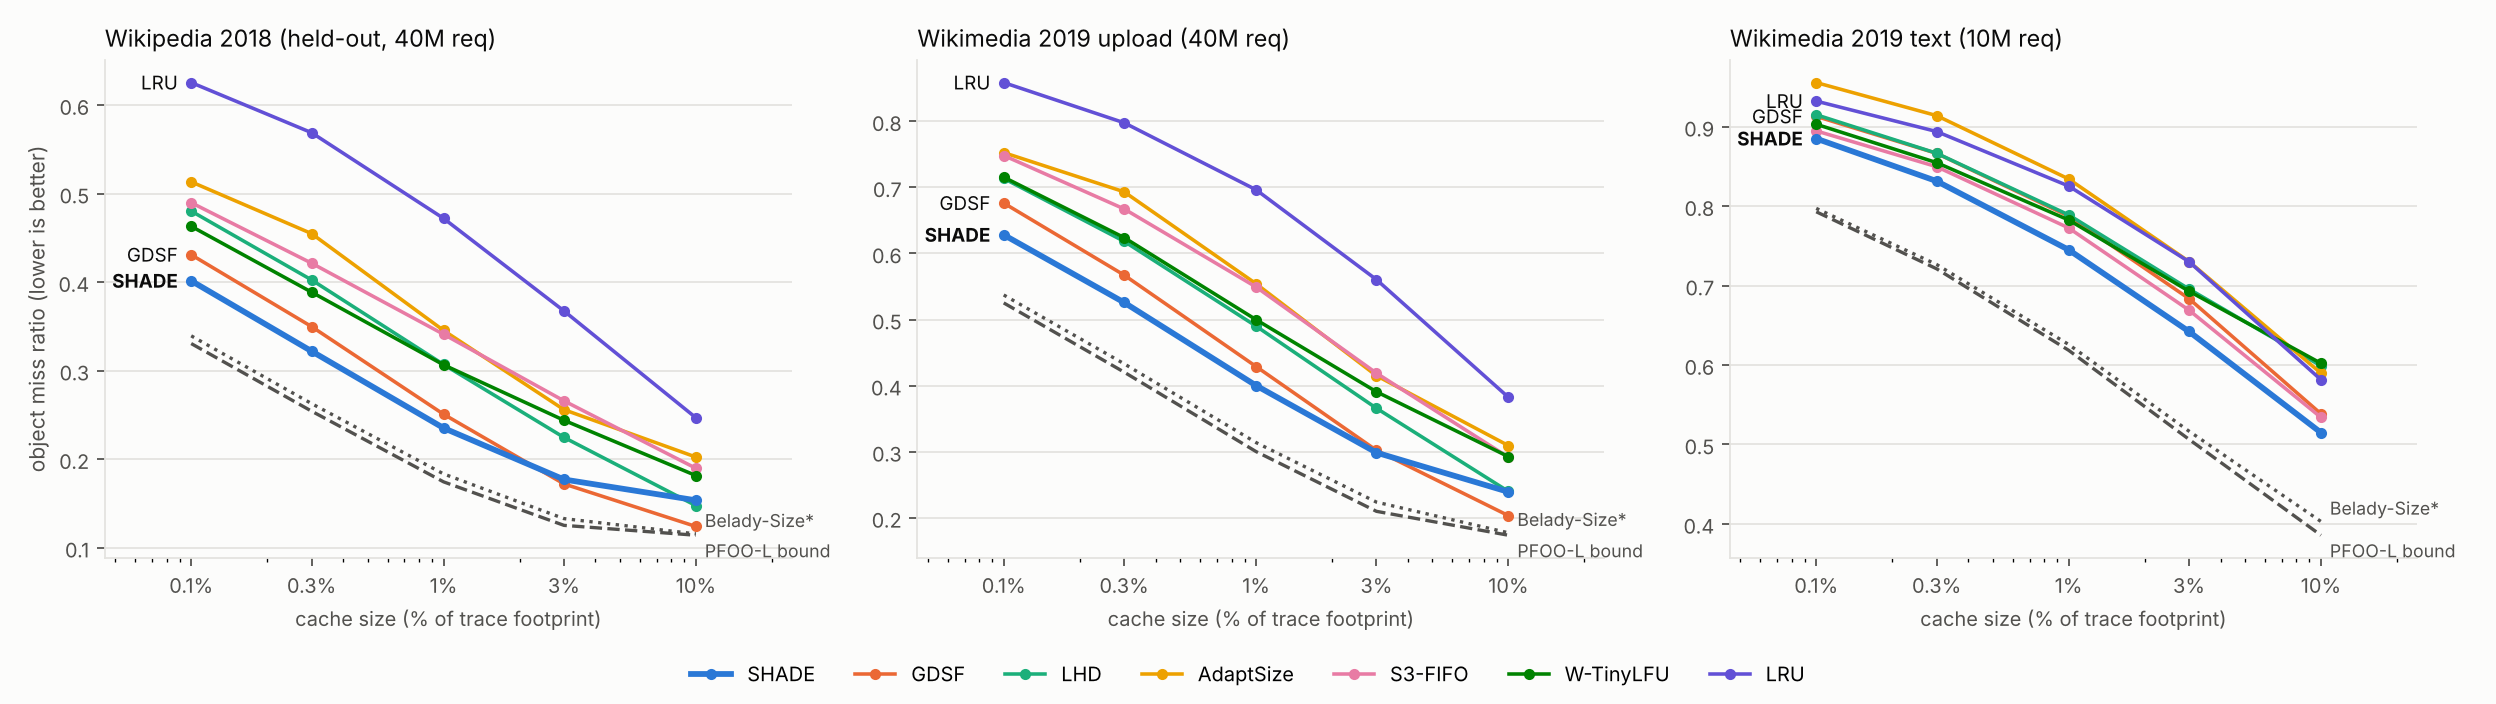
\includegraphics[width=\textwidth]{lab_miss_ratio.png}
\caption{Object miss ratio versus cache size on the three held-out traces (lower is better). Dashed lines: PFOO-L
bound and Belady-Size (offline). Single run per point.}
\label{fig:miss}
\end{figure*}

\begin{table}[t]
\centering
\caption{Object miss ratio: SHADE vs.\ best of eight baselines. $\Delta$ = relative change in misses (negative =
SHADE better).}\label{tab:main}
\setlength{\tabcolsep}{4pt}
\begin{tabular}{@{}llrrrr@{}}
\toprule
Trace & Cache & SHADE & Best & Which & $\Delta$ \\
\midrule
\multirow{5}{*}{W18 test} & 0.1\% & 0.402 & 0.431 & GDSF & $-6.8\%$ \\
 & 0.3\% & 0.322 & 0.350 & GDSF & $-7.9\%$ \\
 & 1\% & 0.235 & 0.251 & GDSF & $-6.2\%$ \\
 & 3\% & 0.177 & 0.172 & GDSF & $+2.9\%$ \\
 & 10\% & 0.154 & 0.124 & GDSF & $+23.8\%$ \\
\midrule
\multirow{5}{*}{W19 upload} & 0.1\% & 0.628 & 0.676 & GDSF & $-7.1\%$ \\
 & 0.3\% & 0.526 & 0.567 & GDSF & $-7.3\%$ \\
 & 1\% & 0.400 & 0.429 & GDSF & $-6.7\%$ \\
 & 3\% & 0.299 & 0.302 & GDSF & $-1.1\%$ \\
 & 10\% & 0.239 & 0.204 & GDSF & $+17.7\%$ \\
\midrule
\multirow{5}{*}{W19 text} & 0.1\% & 0.885 & 0.895 & S3-FIFO & $-1.1\%$ \\
 & 0.3\% & 0.832 & 0.850 & S3-FIFO & $-2.1\%$ \\
 & 1\% & 0.745 & 0.773 & S3-FIFO & $-3.6\%$ \\
 & 3\% & 0.642 & 0.669 & S3-FIFO & $-4.0\%$ \\
 & 10\% & 0.515 & 0.534 & S3-FIFO & $-3.6\%$ \\
\bottomrule
\end{tabular}
\end{table}

SHADE has the lowest miss ratio in 12 of 15 held-out settings. On the two media traces it has 6--8\% fewer misses
than GDSF at 0.1--1\% cache. Three of the 12 wins are small: $-1.1\%$ (W19 upload, 3\%) and $-1.1\%$/$-2.1\%$ (W19
text, 0.1\%/0.3\%). Without variance estimates we cannot say whether margins of this size would survive repeated
runs. Compared with LRU, SHADE removes 5--52\% of misses.

\textbf{Where SHADE loses.} At 10\% cache SHADE is 18--24\% worse than GDSF on both media traces, and at 3\% it is
2.9\% worse on W18. The development slice already showed a loss at 10\% ($+3.0\%$); the held-out loss is much
larger. We did not change the method after seeing it. We have not diagnosed the cause; a plausible hypothesis is that
the exchange-test admission is too conservative when the cache is large enough to hold many objects with long reuse
times, but we have not tested this.

\textbf{Gap to the bound.} At 1\% cache SHADE's miss ratio is 0.235 vs.\ 0.174 for PFOO-L on W18 and 0.745 vs.\ 0.619
on W19 text, so a substantial gap remains. PFOO-L is a relaxation, so part of that gap may not be achievable by any
policy.

\subsection{Byte miss ratio}
SHADE optimises object hits and is not competitive on bytes. The byte variant SHADE-B (rank $= I(c_x,a_x)$, i.e.\ without dividing by $s_x$) beats the best baseline, S3-FIFO, in 10 of 15 held-out settings, but only by 0.3--1.9\%, and loses by
0.1--0.6\% at 0.1--0.3\% cache. We consider this result inconclusive given the single-run design.

\subsection{Ablation}\label{sec:ablation}
Fig.~\ref{fig:abl} removes one component at a time at 1\% cache.

\begin{figure*}[t]
\centering
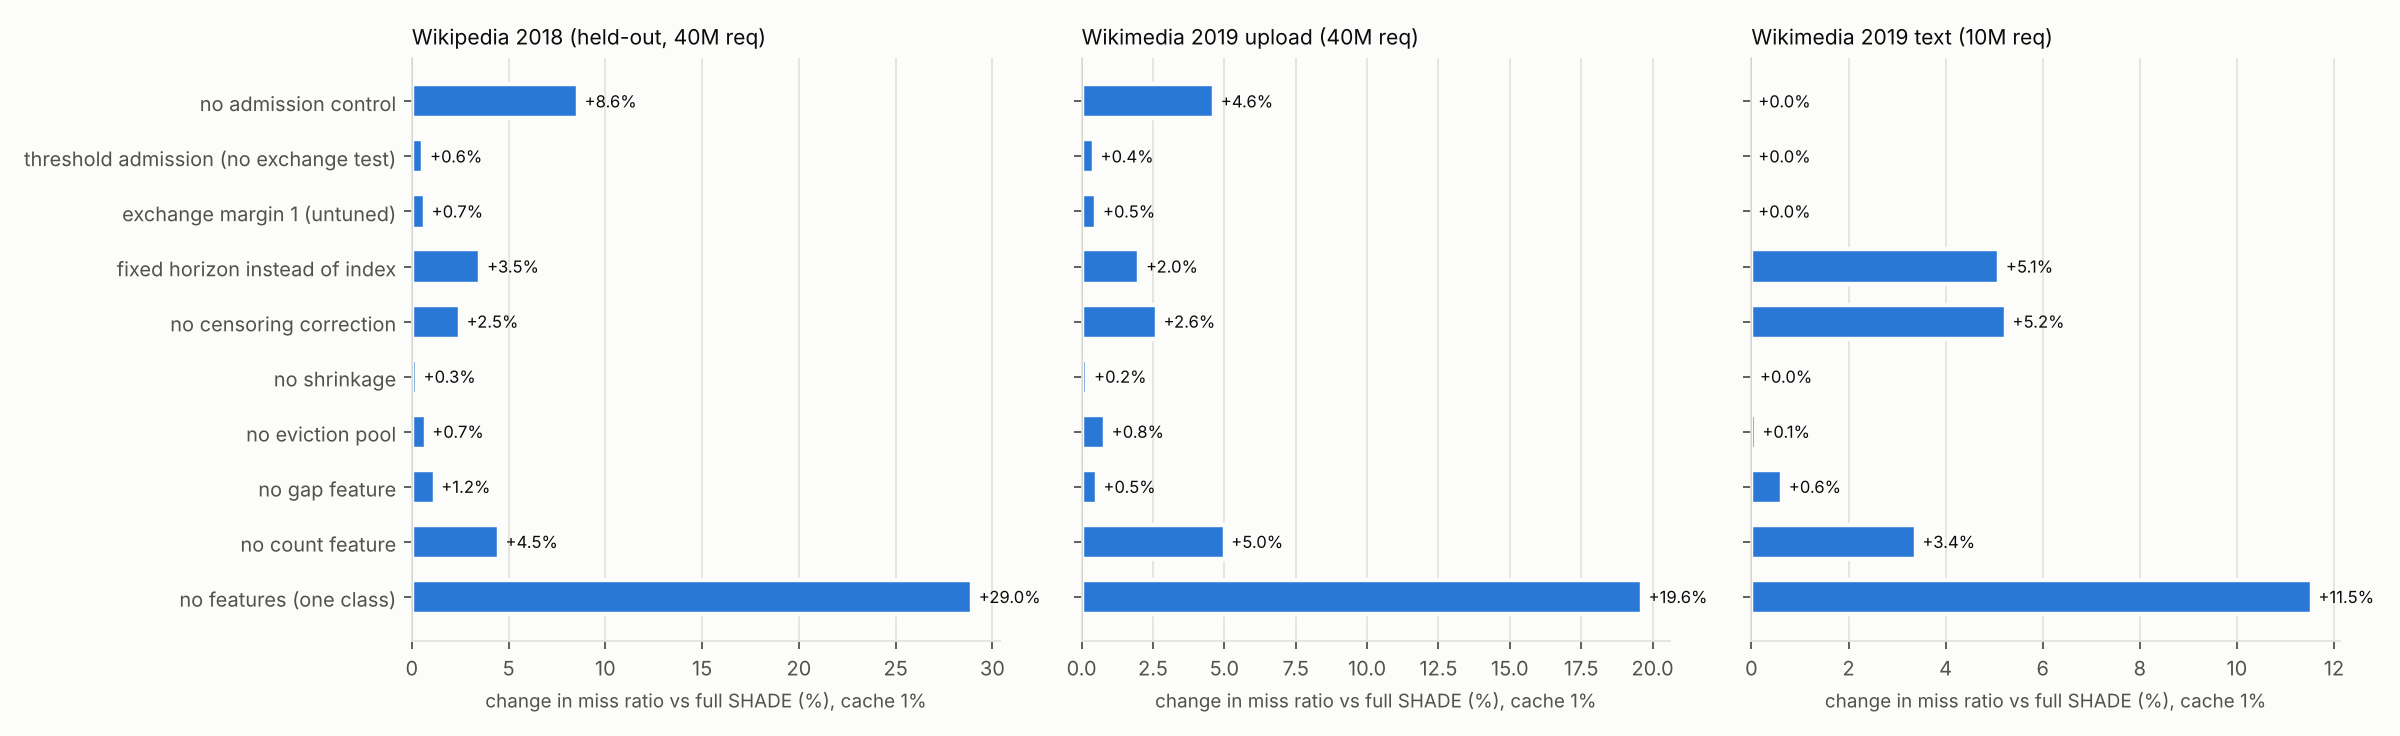
\includegraphics[width=\textwidth]{lab_ablation.png}
\caption{Ablation at 1\% cache: increase in object miss ratio when one component is removed (larger = component
matters more).}
\label{fig:abl}
\end{figure*}

\begin{itemize}
\item \textbf{Features matter most.} Using one class for all objects raises misses by 11.5--29\%. The request-count
feature alone accounts for 3.4--5.0\%.
\item \textbf{Censoring correction and the optimal-stopping index} each contribute 2--5\%.
\item \textbf{Admission} matters on the media traces (no admission: $+4.6\%$ and $+8.6\%$) and not at all on the text
trace ($0.0\%$), where the admission test apparently never rejects.
\item \textbf{The exchange test itself contributes little.} Replacing it with a simple threshold admission costs only
0.4--0.6\%, and an untuned margin $m=1$ costs 0.5--0.7\%. Most of the admission benefit comes from having a good
density estimate for uncached objects, not from the exchange formulation.
\item Shrinkage and the eviction pool each contribute under 1\%.
\end{itemize}

%=====================================================================
\section{A Negative Result: Exact Planning on Real Traffic}\label{sec:v1}
The v1 planner (PACK-DP) solved an exact knapsack each epoch on forecast popularity, combining a Hedge ensemble of
forecasters, a Poisson burst detector, and an admission penalty. On five synthetic workloads it beat every deployable
baseline in 150 of 150 paired comparisons (5 seeds, parameters tuned on separate seeds). When replayed on a real
Wikipedia trace it ranked fourth of six policies. We did not keep the result files for that run, so this number is
not reproducible from the repository and should be read as an observation, not a measured result. Our explanation
is that real traffic is dominated by one-time requests, which an epoch forecaster cannot anticipate, and that
prefetching planned contents wasted bandwidth. Two lessons carried into SHADE: learn from the real request stream,
and treat admission as seriously as eviction. The broader lesson is that synthetic workloads overstated the value of
exact optimisation; in v1, forecast error (4--8 points of captured benefit) already exceeded the greedy-vs-exact
solver gap ($\le0.1$ points) at the default cache size.

%=====================================================================
\section{Threats to Validity}
\begin{itemize}
\item \textbf{No variance estimates.} One run per setting; small margins may not be significant.
\item \textbf{One operator.} All traces come from Wikimedia; results may not transfer to commercial CDNs, video
platforms or other mixes.
\item \textbf{Baseline fidelity.} Seven of eight baselines are our reimplementations, not validated against
reference outputs, and use default parameters.
\item \textbf{Missing baselines.} No learned policies (LRB \cite{lrb}, GL-Cache, 3L-Cache).
\item \textbf{Simulation only.} Logical time, no wall-clock bursts, no TTLs, range requests or request coalescing;
no deployment.
\item \textbf{Freeze evidence.} Only the commit order supports the frozen-method claim.
\item \textbf{Metadata cost.} SHADE stores more state than the simplest baselines; the comparison does not charge
that metadata against cache capacity.
\item \textbf{Novelty.} We did not perform an exhaustive literature search.
\end{itemize}

%=====================================================================
\section{Conclusion}
Viewing caching as a fractional knapsack over reuse intervals gives a clear target: keep what beats a shadow price.
SHADE approximates that rule online and, on three held-out Wikimedia traces, has fewer misses than eight
reimplemented baselines at small and medium cache sizes. It loses clearly to GDSF at large caches, its byte variant
is only marginally better than S3-FIFO, and the evaluation is single-run and single-operator. The ablation suggests
the main value comes from policy-independent, censoring-corrected reuse statistics with good features, rather than
from the exchange-test formulation. Next steps: repeated runs with confidence intervals, learned baselines, traces
from other operators, and a diagnosis of the large-cache loss.

\section*{Reproducibility}
Code, results (JSON) and scripts are in the project repository. \texttt{make lab-test} runs the 460 checks;
\texttt{make traces} and \texttt{make heldout} download the traces and rerun the evaluation (about 1.5\,h on 4 cores).

\section*{Acknowledgment}
Parts of the code and of this manuscript were written with the assistance of an AI coding assistant (Claude, by
Anthropic). The authors reviewed the outputs and are responsible for all content.

\begin{thebibliography}{00}
\bibitem{pfoo} D.~S. Berger, N.~Beckmann, and M.~Harchol-Balter, ``Practical bounds on optimal caching with variable
object sizes,'' \emph{Proc. ACM Meas. Anal. Comput. Syst. (SIGMETRICS)}, vol.~2, no.~2, 2018.
\bibitem{belady} L.~A. Belady, ``A study of replacement algorithms for a virtual-storage computer,'' \emph{IBM Syst.
J.}, vol.~5, no.~2, pp.~78--101, 1966.
\bibitem{sleator} D.~D. Sleator and R.~E. Tarjan, ``Amortized efficiency of list update and paging rules,''
\emph{Commun. ACM}, vol.~28, no.~2, pp.~202--208, 1985.
\bibitem{gdsf} L.~Cherkasova, ``Improving WWW proxies performance with Greedy-Dual-Size-Frequency caching policy,''
HP Labs, Tech. Rep. HPL-98-69, 1998.
\bibitem{adaptsize} D.~S. Berger, R.~K. Sitaraman, and M.~Harchol-Balter, ``AdaptSize: Orchestrating the hot object
memory cache in a content delivery network,'' in \emph{Proc. USENIX NSDI}, 2017.
\bibitem{lhd} N.~Beckmann, H.~Chen, and A.~Cidon, ``LHD: Improving cache hit rate by maximizing hit density,'' in
\emph{Proc. USENIX NSDI}, 2018.
\bibitem{tinylfu} G.~Einziger, R.~Friedman, and B.~Manes, ``TinyLFU: A highly efficient cache admission policy,''
\emph{ACM Trans. Storage}, vol.~13, no.~4, 2017.
\bibitem{s3fifo} J.~Yang, Y.~Zhang, Z.~Qiu, Y.~Yue, and R.~Vinayak, ``FIFO queues are all you need for cache
eviction,'' in \emph{Proc. ACM SOSP}, 2023.
\bibitem{sieve} Y.~Zhang, J.~Yang, Y.~Yue, Y.~Vigfusson, and K.~V. Rashmi, ``SIEVE is simpler than LRU: An efficient
turn-key eviction algorithm for web caches,'' in \emph{Proc. USENIX NSDI}, 2024.
\bibitem{lrb} Z.~Song, D.~S. Berger, K.~Li, and W.~Lloyd, ``Learning relaxed Belady for content distribution network
caching,'' in \emph{Proc. USENIX NSDI}, 2020.
\bibitem{akamai} B.~M. Maggs and R.~K. Sitaraman, ``Algorithmic nuggets in content delivery,'' \emph{ACM SIGCOMM
Comput. Commun. Rev.}, vol.~45, no.~3, 2015.
\bibitem{hirschberg} D.~S. Hirschberg, ``A linear space algorithm for computing maximal common subsequences,''
\emph{Commun. ACM}, vol.~18, no.~6, pp.~341--343, 1975.
\bibitem{mt} S.~Martello and P.~Toth, ``An upper bound for the zero-one knapsack problem and a branch and bound
algorithm,'' \emph{Eur. J. Oper. Res.}, vol.~1, pp.~169--175, 1977.
\bibitem{ibarra} O.~H. Ibarra and C.~E. Kim, ``Fast approximation algorithms for the knapsack and sum of subset
problems,'' \emph{J. ACM}, vol.~22, no.~4, pp.~463--468, 1975.
\end{thebibliography}

\end{document}
